\section{meshmorph.h File Reference}
\label{meshmorph_8h}\index{meshmorph.h@{meshmorph.h}}
{\tt \#include $<$cmath$>$}\par
{\tt \#include $<$iostream$>$}\par
{\tt \#include $<$ext/hash\_\-map$>$}\par
{\tt \#include $<$ext/hash\_\-set$>$}\par
{\tt \#include $<$map$>$}\par
{\tt \#include $<$set$>$}\par
{\tt \#include $<$string$>$}\par
{\tt \#include $<$vector$>$}\par


Include dependency graph for meshmorph.h:\begin{figure}[H]
\begin{center}
\leavevmode
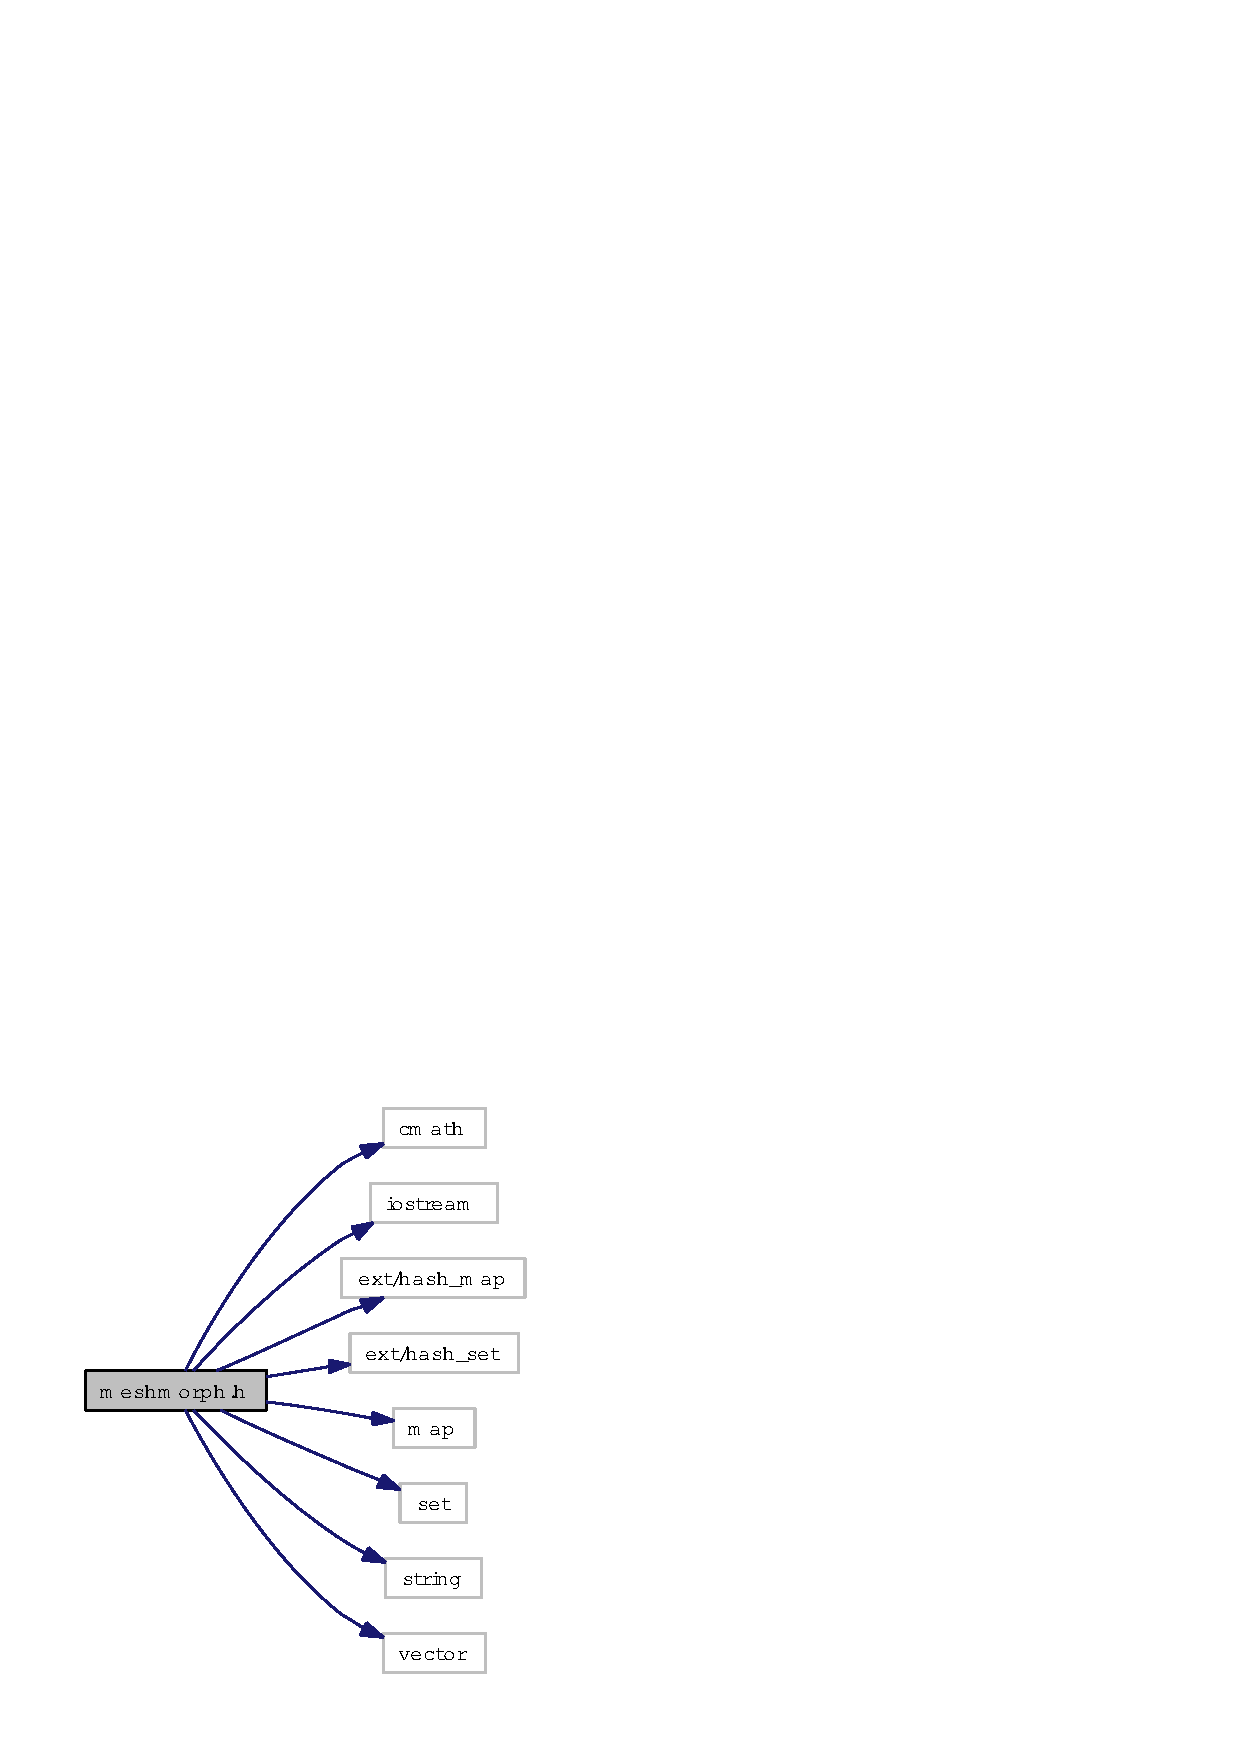
\includegraphics[width=128pt]{meshmorph_8h__incl}
\end{center}
\end{figure}


This graph shows which files directly or indirectly include this file:\begin{figure}[H]
\begin{center}
\leavevmode
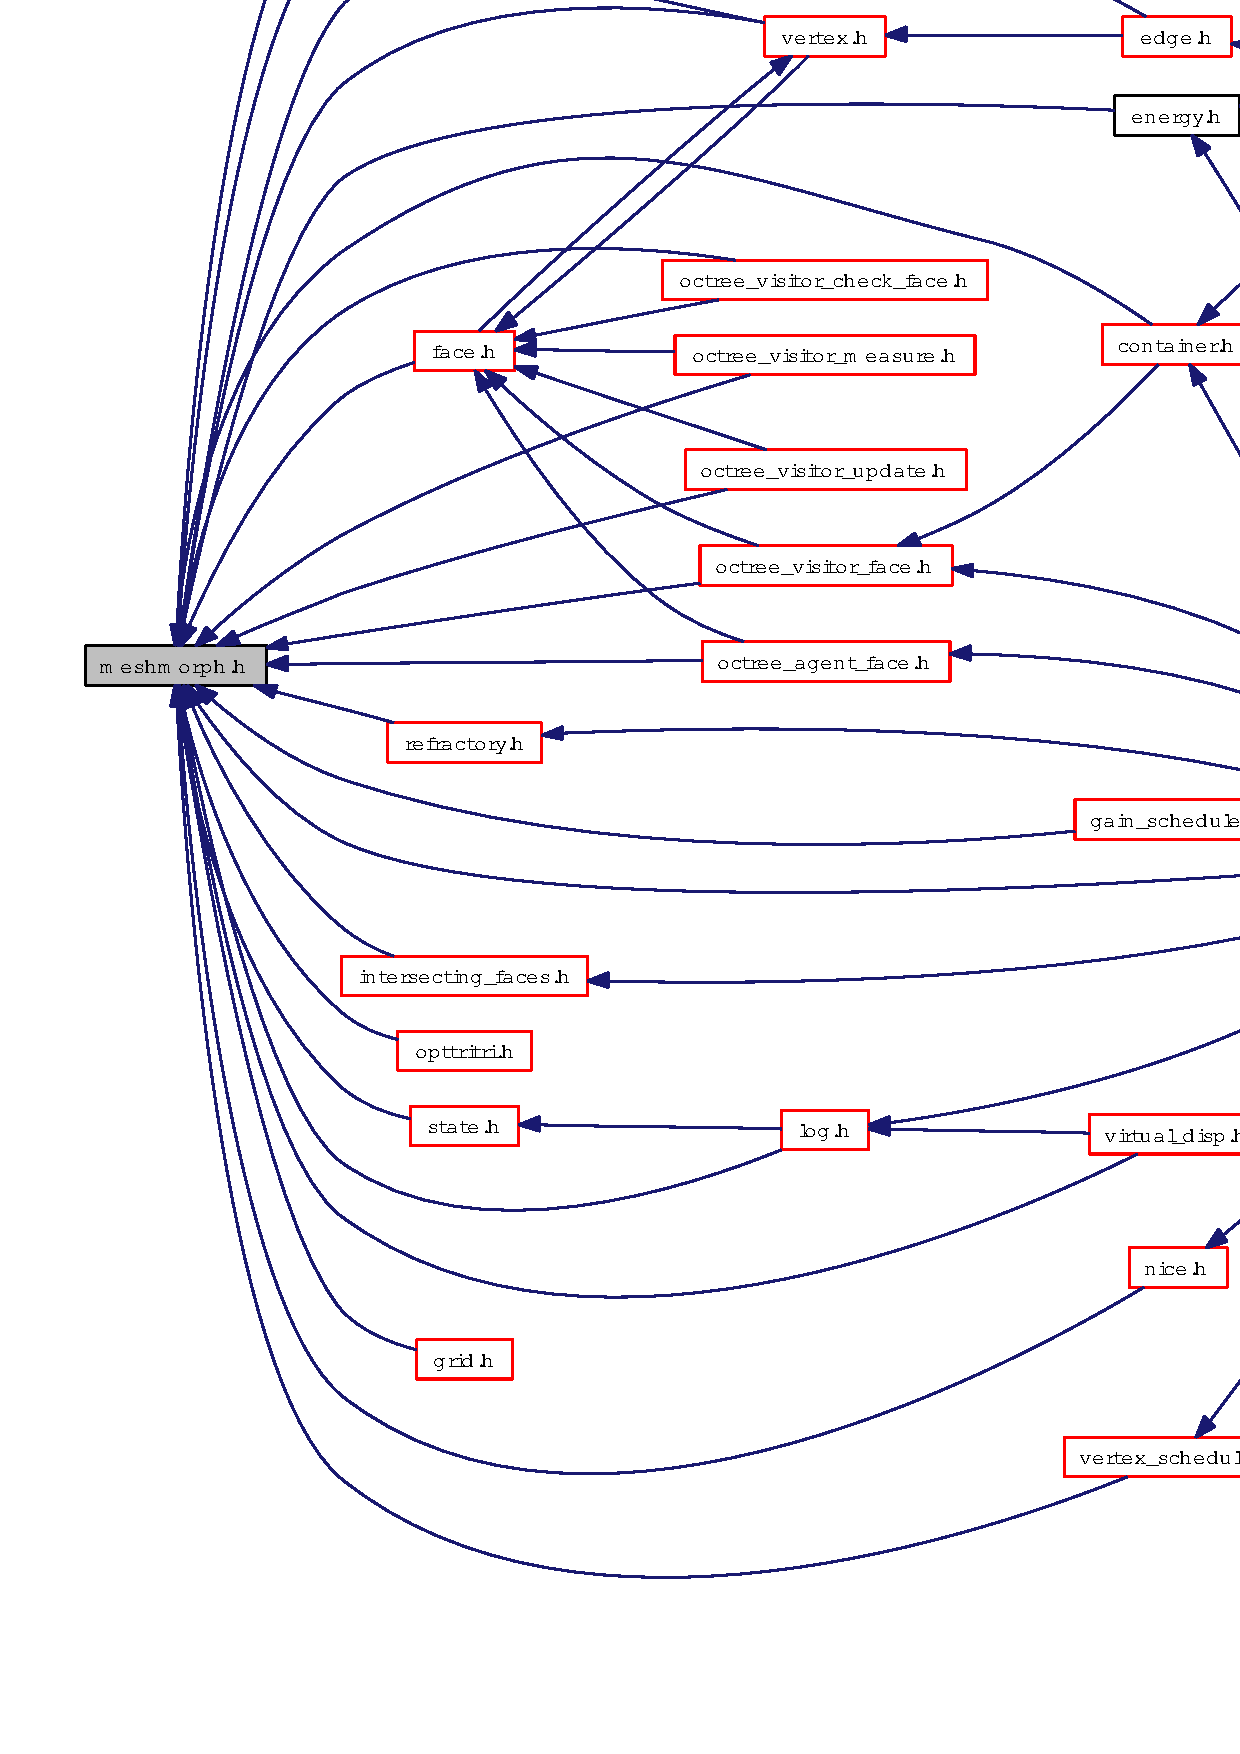
\includegraphics[width=376pt]{meshmorph_8h__dep__incl}
\end{center}
\end{figure}
\subsection*{Classes}
\begin{CompactItemize}
\item 
struct {\bf f\_\-hash}
\item 
struct {\bf v\_\-hash}
\item 
struct {\bf e\_\-hash}
\item 
struct {\bf vector3}
\item 
struct {\bf Minmax}
\item 
struct {\bf result}
\end{CompactItemize}
\subsection*{Defines}
\begin{CompactItemize}
\item 
\#define {\bf MESHMORPH\_\-H}~1
\end{CompactItemize}
\subsection*{Typedefs}
\begin{CompactItemize}
\item 
typedef unsigned long int {\bf u4}
\item 
typedef unsigned char {\bf u1}
\item 
typedef std::equal\_\-to$<$ const {\bf Face} $\ast$ $>$ {\bf eqf}
\item 
typedef std::equal\_\-to$<$ const {\bf Edge} $\ast$ $>$ {\bf eqe}
\item 
typedef std::equal\_\-to$<$ const {\bf Vertex} $\ast$ $>$ {\bf eqv}
\item 
typedef std::less$<$ const {\bf Edge} $\ast$ $>$ {\bf lte}
\item 
typedef std::less$<$ const {\bf Object} $\ast$ $>$ {\bf lto}
\item 
typedef std::less$<$ const {\bf Vertex} $\ast$ $>$ {\bf ltv}
\item 
typedef std::less$<$ const {\bf Face} $\ast$ $>$ {\bf ltf}
\item 
typedef std::less$<$ const std::string $>$ {\bf lts}
\item 
typedef std::less$<$ const double $>$ {\bf ltd}
\item 
typedef std::vector$<$ {\bf Vertex} $>$ {\bf vec\_\-v}
\item 
typedef std::vector$<$ {\bf Vertex} $>$::iterator {\bf v\_\-it}
\item 
typedef std::vector$<$ {\bf Vertex} $>$::const\_\-iterator {\bf v\_\-cit}
\item 
typedef std::vector$<$ {\bf Face} $>$ {\bf vec\_\-f}
\item 
typedef std::vector$<$ {\bf Face} $>$::iterator {\bf f\_\-it}
\item 
typedef std::vector$<$ {\bf Face} $>$::const\_\-iterator {\bf f\_\-cit}
\item 
typedef std::vector$<$ {\bf Edge} $>$ {\bf vec\_\-e}
\item 
typedef std::vector$<$ {\bf Edge} $>$::iterator {\bf e\_\-it}
\item 
typedef std::vector$<$ {\bf Edge} $>$::const\_\-iterator {\bf e\_\-cit}
\item 
typedef std::vector$<$ {\bf Object} $>$ {\bf vec\_\-o}
\item 
typedef std::vector$<$ {\bf Object} $>$::iterator {\bf o\_\-it}
\item 
typedef std::vector$<$ {\bf Object} $>$::const\_\-iterator {\bf o\_\-cit}
\item 
typedef std::vector$<$ {\bf Vertex} $\ast$ $>$ {\bf vec\_\-vp}
\item 
typedef std::vector$<$ {\bf Vertex} $\ast$ $>$::iterator {\bf vp\_\-it}
\item 
typedef std::vector$<$ {\bf Vertex} $\ast$ $>$::const\_\-iterator {\bf vp\_\-cit}
\item 
typedef std::vector$<$ {\bf Face} $\ast$ $>$ {\bf vec\_\-fp}
\item 
typedef std::vector$<$ {\bf Face} $\ast$ $>$::iterator {\bf fp\_\-it}
\item 
typedef std::vector$<$ {\bf Face} $\ast$ $>$::const\_\-iterator {\bf fp\_\-cit}
\item 
typedef std::vector$<$ {\bf Edge} $\ast$ $>$ {\bf vec\_\-ep}
\item 
typedef std::vector$<$ {\bf Edge} $\ast$ $>$::iterator {\bf ep\_\-it}
\item 
typedef std::vector$<$ {\bf Edge} $\ast$ $>$::const\_\-iterator {\bf ep\_\-cit}
\item 
typedef std::vector$<$ {\bf Object} $\ast$ $>$ {\bf vec\_\-op}
\item 
typedef std::vector$<$ {\bf Object} $\ast$ $>$::iterator {\bf op\_\-it}
\item 
typedef std::vector$<$ int $>$ {\bf vec\_\-i}
\item 
typedef std::vector$<$ int $>$::iterator {\bf i\_\-it}
\item 
typedef std::vector$<$ double $>$ {\bf vec\_\-d}
\item 
typedef std::vector$<$ double $>$::iterator {\bf d\_\-it}
\item 
typedef std::vector$<$ double $>$::const\_\-iterator {\bf d\_\-cit}
\item 
typedef std::vector$<$ std::string $>$ {\bf vec\_\-s}
\item 
typedef std::set$<$ std::string, {\bf lts} $>$ {\bf s\_\-set}
\item 
typedef std::set$<$ std::string, {\bf lts} $>$::iterator {\bf ss\_\-it}
\item 
typedef std::set$<$ {\bf Edge} $\ast$, {\bf lte} $>$ {\bf e\_\-set}
\item 
typedef std::set$<$ {\bf Edge} $\ast$, {\bf lte} $>$::iterator {\bf es\_\-it}
\item 
typedef std::set$<$ {\bf Vertex} $\ast$, {\bf ltv} $>$ {\bf v\_\-set}
\item 
typedef std::set$<$ {\bf Vertex} $\ast$, {\bf ltv} $>$::iterator {\bf vs\_\-it}
\item 
typedef std::set$<$ {\bf Face} $\ast$, {\bf ltf} $>$ {\bf f\_\-set}
\item 
typedef std::set$<$ {\bf Face} $\ast$, {\bf ltf} $>$::iterator {\bf fs\_\-it}
\item 
typedef \_\-\_\-gnu\_\-cxx::hash\_\-set$<$ {\bf Vertex} $\ast$, {\bf v\_\-hash}, {\bf eqv} $>$ {\bf hashset\_\-v}
\item 
typedef std::map$<$ std::string, {\bf Edge} $\ast$, {\bf lts} $>$ {\bf map\_\-s\_\-ep}
\item 
typedef \_\-\_\-gnu\_\-cxx::hash\_\-map$<$ {\bf Vertex} $\ast$, int, {\bf v\_\-hash}, {\bf eqv} $>$ {\bf hmap\_\-v}
\item 
typedef \_\-\_\-gnu\_\-cxx::hash\_\-map$<$ {\bf Vertex} $\ast$, int, {\bf v\_\-hash}, {\bf eqv} $>$::const\_\-iterator {\bf vhm\_\-cit}
\end{CompactItemize}
\subsection*{Functions}
\begin{CompactItemize}
\item 
bool {\bf distinguishable} (double a, double b, double epsilon)
\item 
bool {\bf distinguishable} (double a, double b)
\item 
bool {\bf check\-Int\-Size} (void)
\end{CompactItemize}


\subsection{Define Documentation}
\index{meshmorph.h@{meshmorph.h}!MESHMORPH_H@{MESHMORPH\_\-H}}
\index{MESHMORPH_H@{MESHMORPH\_\-H}!meshmorph.h@{meshmorph.h}}
\subsubsection{\setlength{\rightskip}{0pt plus 5cm}\#define MESHMORPH\_\-H~1}\label{meshmorph_8h_71120f21a107c5b75048614176bf8599}




\subsection{Typedef Documentation}
\index{meshmorph.h@{meshmorph.h}!d_cit@{d\_\-cit}}
\index{d_cit@{d\_\-cit}!meshmorph.h@{meshmorph.h}}
\subsubsection{\setlength{\rightskip}{0pt plus 5cm}typedef std::vector$<$double$>$::const\_\-iterator {\bf d\_\-cit}}\label{meshmorph_8h_2b0b40988a1846cebbeba82928d904a0}


\index{meshmorph.h@{meshmorph.h}!d_it@{d\_\-it}}
\index{d_it@{d\_\-it}!meshmorph.h@{meshmorph.h}}
\subsubsection{\setlength{\rightskip}{0pt plus 5cm}typedef std::vector$<$double$>$::iterator {\bf d\_\-it}}\label{meshmorph_8h_e48600948a78e106d03c76c264304228}


\index{meshmorph.h@{meshmorph.h}!e_cit@{e\_\-cit}}
\index{e_cit@{e\_\-cit}!meshmorph.h@{meshmorph.h}}
\subsubsection{\setlength{\rightskip}{0pt plus 5cm}typedef std::vector$<${\bf Edge}$>$::const\_\-iterator {\bf e\_\-cit}}\label{meshmorph_8h_22d8871843ac79d4b0e9c2fed01fb62b}


\index{meshmorph.h@{meshmorph.h}!e_it@{e\_\-it}}
\index{e_it@{e\_\-it}!meshmorph.h@{meshmorph.h}}
\subsubsection{\setlength{\rightskip}{0pt plus 5cm}typedef std::vector$<${\bf Edge}$>$::iterator {\bf e\_\-it}}\label{meshmorph_8h_1db3950949af5e08df041e08dbd14556}


\index{meshmorph.h@{meshmorph.h}!e_set@{e\_\-set}}
\index{e_set@{e\_\-set}!meshmorph.h@{meshmorph.h}}
\subsubsection{\setlength{\rightskip}{0pt plus 5cm}typedef std::set$<${\bf Edge}$\ast$,{\bf lte}$>$ {\bf e\_\-set}}\label{meshmorph_8h_00e760a04acb1a5623bd79189a3d5e44}


\index{meshmorph.h@{meshmorph.h}!ep_cit@{ep\_\-cit}}
\index{ep_cit@{ep\_\-cit}!meshmorph.h@{meshmorph.h}}
\subsubsection{\setlength{\rightskip}{0pt plus 5cm}typedef std::vector$<${\bf Edge}$\ast$$>$::const\_\-iterator {\bf ep\_\-cit}}\label{meshmorph_8h_7bbde133ac39ecfc284c91b3da140e56}


\index{meshmorph.h@{meshmorph.h}!ep_it@{ep\_\-it}}
\index{ep_it@{ep\_\-it}!meshmorph.h@{meshmorph.h}}
\subsubsection{\setlength{\rightskip}{0pt plus 5cm}typedef std::vector$<${\bf Edge}$\ast$$>$::iterator {\bf ep\_\-it}}\label{meshmorph_8h_2c2a5a920658be1c063b7bb97132ad02}


\index{meshmorph.h@{meshmorph.h}!eqe@{eqe}}
\index{eqe@{eqe}!meshmorph.h@{meshmorph.h}}
\subsubsection{\setlength{\rightskip}{0pt plus 5cm}typedef std::equal\_\-to$<$const {\bf Edge} $\ast$$>$ {\bf eqe}}\label{meshmorph_8h_d000fbd6ebbfd4ec6a1091b0fdade132}


\index{meshmorph.h@{meshmorph.h}!eqf@{eqf}}
\index{eqf@{eqf}!meshmorph.h@{meshmorph.h}}
\subsubsection{\setlength{\rightskip}{0pt plus 5cm}typedef std::equal\_\-to$<$const {\bf Face} $\ast$$>$ {\bf eqf}}\label{meshmorph_8h_60b006c4da96f6f67a50b4dd7a1c14bd}


\index{meshmorph.h@{meshmorph.h}!eqv@{eqv}}
\index{eqv@{eqv}!meshmorph.h@{meshmorph.h}}
\subsubsection{\setlength{\rightskip}{0pt plus 5cm}typedef std::equal\_\-to$<$const {\bf Vertex} $\ast$$>$ {\bf eqv}}\label{meshmorph_8h_5e4c69ea7515d6d451847631e6db1a04}


\index{meshmorph.h@{meshmorph.h}!es_it@{es\_\-it}}
\index{es_it@{es\_\-it}!meshmorph.h@{meshmorph.h}}
\subsubsection{\setlength{\rightskip}{0pt plus 5cm}typedef std::set$<${\bf Edge}$\ast$,{\bf lte}$>$::iterator {\bf es\_\-it}}\label{meshmorph_8h_be3f719aca3e5fff13f0f0384815ca50}


\index{meshmorph.h@{meshmorph.h}!f_cit@{f\_\-cit}}
\index{f_cit@{f\_\-cit}!meshmorph.h@{meshmorph.h}}
\subsubsection{\setlength{\rightskip}{0pt plus 5cm}typedef std::vector$<${\bf Face}$>$::const\_\-iterator {\bf f\_\-cit}}\label{meshmorph_8h_1bdf0f72f7c8cbe704a0f6b64be07f6b}


\index{meshmorph.h@{meshmorph.h}!f_it@{f\_\-it}}
\index{f_it@{f\_\-it}!meshmorph.h@{meshmorph.h}}
\subsubsection{\setlength{\rightskip}{0pt plus 5cm}typedef std::vector$<${\bf Face}$>$::iterator {\bf f\_\-it}}\label{meshmorph_8h_a19fd10324725dd9216be23ee875011e}


\index{meshmorph.h@{meshmorph.h}!f_set@{f\_\-set}}
\index{f_set@{f\_\-set}!meshmorph.h@{meshmorph.h}}
\subsubsection{\setlength{\rightskip}{0pt plus 5cm}typedef std::set$<${\bf Face}$\ast$,{\bf ltf}$>$ {\bf f\_\-set}}\label{meshmorph_8h_18c3a5c9149f71028e8356a5f59979c1}


\index{meshmorph.h@{meshmorph.h}!fp_cit@{fp\_\-cit}}
\index{fp_cit@{fp\_\-cit}!meshmorph.h@{meshmorph.h}}
\subsubsection{\setlength{\rightskip}{0pt plus 5cm}typedef std::vector$<${\bf Face}$\ast$$>$::const\_\-iterator {\bf fp\_\-cit}}\label{meshmorph_8h_8d2bcc70fbd9a2cca7eecb128703e8c7}


\index{meshmorph.h@{meshmorph.h}!fp_it@{fp\_\-it}}
\index{fp_it@{fp\_\-it}!meshmorph.h@{meshmorph.h}}
\subsubsection{\setlength{\rightskip}{0pt plus 5cm}typedef std::vector$<${\bf Face}$\ast$$>$::iterator {\bf fp\_\-it}}\label{meshmorph_8h_c65901c49115edae93d689df5a5e2078}


\index{meshmorph.h@{meshmorph.h}!fs_it@{fs\_\-it}}
\index{fs_it@{fs\_\-it}!meshmorph.h@{meshmorph.h}}
\subsubsection{\setlength{\rightskip}{0pt plus 5cm}typedef std::set$<${\bf Face}$\ast$,{\bf ltf}$>$::iterator {\bf fs\_\-it}}\label{meshmorph_8h_ac3d66c96f82288309b43040bf91b2d0}


\index{meshmorph.h@{meshmorph.h}!hashset_v@{hashset\_\-v}}
\index{hashset_v@{hashset\_\-v}!meshmorph.h@{meshmorph.h}}
\subsubsection{\setlength{\rightskip}{0pt plus 5cm}typedef \_\-\_\-gnu\_\-cxx::hash\_\-set$<${\bf Vertex}$\ast$,{\bf v\_\-hash},{\bf eqv}$>$ {\bf hashset\_\-v}}\label{meshmorph_8h_274b35739790732fd62f8771c082edb0}


\index{meshmorph.h@{meshmorph.h}!hmap_v@{hmap\_\-v}}
\index{hmap_v@{hmap\_\-v}!meshmorph.h@{meshmorph.h}}
\subsubsection{\setlength{\rightskip}{0pt plus 5cm}typedef \_\-\_\-gnu\_\-cxx::hash\_\-map$<${\bf Vertex}$\ast$,int,{\bf v\_\-hash},{\bf eqv}$>$ {\bf hmap\_\-v}}\label{meshmorph_8h_98cba187ef21b37be895460edbcbbe4d}


\index{meshmorph.h@{meshmorph.h}!i_it@{i\_\-it}}
\index{i_it@{i\_\-it}!meshmorph.h@{meshmorph.h}}
\subsubsection{\setlength{\rightskip}{0pt plus 5cm}typedef std::vector$<$int$>$::iterator {\bf i\_\-it}}\label{meshmorph_8h_8824401dc94595ec38aa0c359a8cf6c0}


\index{meshmorph.h@{meshmorph.h}!ltd@{ltd}}
\index{ltd@{ltd}!meshmorph.h@{meshmorph.h}}
\subsubsection{\setlength{\rightskip}{0pt plus 5cm}typedef std::less$<$const double$>$ {\bf ltd}}\label{meshmorph_8h_8395a7f9a95c868d9f7a2679b7b9c4c6}


\index{meshmorph.h@{meshmorph.h}!lte@{lte}}
\index{lte@{lte}!meshmorph.h@{meshmorph.h}}
\subsubsection{\setlength{\rightskip}{0pt plus 5cm}typedef std::less$<$const {\bf Edge} $\ast$$>$ {\bf lte}}\label{meshmorph_8h_d437f18aff14545bb2f4ba6bb223b9f9}


\index{meshmorph.h@{meshmorph.h}!ltf@{ltf}}
\index{ltf@{ltf}!meshmorph.h@{meshmorph.h}}
\subsubsection{\setlength{\rightskip}{0pt plus 5cm}typedef std::less$<$const {\bf Face} $\ast$$>$ {\bf ltf}}\label{meshmorph_8h_771fe55387804f93885e754766093f69}


\index{meshmorph.h@{meshmorph.h}!lto@{lto}}
\index{lto@{lto}!meshmorph.h@{meshmorph.h}}
\subsubsection{\setlength{\rightskip}{0pt plus 5cm}typedef std::less$<$const {\bf Object} $\ast$$>$ {\bf lto}}\label{meshmorph_8h_8330b10e338fa046ad1547a1e5a2f9c0}


\index{meshmorph.h@{meshmorph.h}!lts@{lts}}
\index{lts@{lts}!meshmorph.h@{meshmorph.h}}
\subsubsection{\setlength{\rightskip}{0pt plus 5cm}typedef std::less$<$const std::string$>$ {\bf lts}}\label{meshmorph_8h_502b03f11852c3daa44121be7f33ba67}


\index{meshmorph.h@{meshmorph.h}!ltv@{ltv}}
\index{ltv@{ltv}!meshmorph.h@{meshmorph.h}}
\subsubsection{\setlength{\rightskip}{0pt plus 5cm}typedef std::less$<$const {\bf Vertex} $\ast$$>$ {\bf ltv}}\label{meshmorph_8h_21e1832a86b3c598ae7cc21040547a49}


\index{meshmorph.h@{meshmorph.h}!map_s_ep@{map\_\-s\_\-ep}}
\index{map_s_ep@{map\_\-s\_\-ep}!meshmorph.h@{meshmorph.h}}
\subsubsection{\setlength{\rightskip}{0pt plus 5cm}typedef std::map$<$std::string,{\bf Edge}$\ast$,{\bf lts}$>$ {\bf map\_\-s\_\-ep}}\label{meshmorph_8h_44f8ecd3bb7785b1b65f8fe86ece7e8f}


\index{meshmorph.h@{meshmorph.h}!o_cit@{o\_\-cit}}
\index{o_cit@{o\_\-cit}!meshmorph.h@{meshmorph.h}}
\subsubsection{\setlength{\rightskip}{0pt plus 5cm}typedef std::vector$<${\bf Object}$>$::const\_\-iterator {\bf o\_\-cit}}\label{meshmorph_8h_bc066bbbef7a11c4ee8fa91ec325d609}


\index{meshmorph.h@{meshmorph.h}!o_it@{o\_\-it}}
\index{o_it@{o\_\-it}!meshmorph.h@{meshmorph.h}}
\subsubsection{\setlength{\rightskip}{0pt plus 5cm}typedef std::vector$<${\bf Object}$>$::iterator {\bf o\_\-it}}\label{meshmorph_8h_ee98e25193e5b352ac2eefbd05ccde6a}


\index{meshmorph.h@{meshmorph.h}!op_it@{op\_\-it}}
\index{op_it@{op\_\-it}!meshmorph.h@{meshmorph.h}}
\subsubsection{\setlength{\rightskip}{0pt plus 5cm}typedef std::vector$<${\bf Object}$\ast$$>$::iterator {\bf op\_\-it}}\label{meshmorph_8h_0f1596befebd38f6b2fe4e7fa62849b9}


\index{meshmorph.h@{meshmorph.h}!s_set@{s\_\-set}}
\index{s_set@{s\_\-set}!meshmorph.h@{meshmorph.h}}
\subsubsection{\setlength{\rightskip}{0pt plus 5cm}typedef std::set$<$std::string,{\bf lts}$>$ {\bf s\_\-set}}\label{meshmorph_8h_b394658db9d9ed70f0e9787f901f9428}


\index{meshmorph.h@{meshmorph.h}!ss_it@{ss\_\-it}}
\index{ss_it@{ss\_\-it}!meshmorph.h@{meshmorph.h}}
\subsubsection{\setlength{\rightskip}{0pt plus 5cm}typedef std::set$<$std::string,{\bf lts}$>$::iterator {\bf ss\_\-it}}\label{meshmorph_8h_e330971fee652d58e1a7fb9154dfbcff}


\index{meshmorph.h@{meshmorph.h}!u1@{u1}}
\index{u1@{u1}!meshmorph.h@{meshmorph.h}}
\subsubsection{\setlength{\rightskip}{0pt plus 5cm}typedef unsigned char {\bf u1}}\label{meshmorph_8h_216a9f8b04b4f0af84a4ca9d1d85a6ca}


\index{meshmorph.h@{meshmorph.h}!u4@{u4}}
\index{u4@{u4}!meshmorph.h@{meshmorph.h}}
\subsubsection{\setlength{\rightskip}{0pt plus 5cm}typedef unsigned long int {\bf u4}}\label{meshmorph_8h_9bcb189c00c284557b4f61c53de32d16}


\index{meshmorph.h@{meshmorph.h}!v_cit@{v\_\-cit}}
\index{v_cit@{v\_\-cit}!meshmorph.h@{meshmorph.h}}
\subsubsection{\setlength{\rightskip}{0pt plus 5cm}typedef std::vector$<${\bf Vertex}$>$::const\_\-iterator {\bf v\_\-cit}}\label{meshmorph_8h_dfa48b42fdac70f72a266296787d27e6}


\index{meshmorph.h@{meshmorph.h}!v_it@{v\_\-it}}
\index{v_it@{v\_\-it}!meshmorph.h@{meshmorph.h}}
\subsubsection{\setlength{\rightskip}{0pt plus 5cm}typedef std::vector$<${\bf Vertex}$>$::iterator {\bf v\_\-it}}\label{meshmorph_8h_3263d78f676958dea30d353e47e8b889}


\index{meshmorph.h@{meshmorph.h}!v_set@{v\_\-set}}
\index{v_set@{v\_\-set}!meshmorph.h@{meshmorph.h}}
\subsubsection{\setlength{\rightskip}{0pt plus 5cm}typedef std::set$<${\bf Vertex}$\ast$,{\bf ltv}$>$ {\bf v\_\-set}}\label{meshmorph_8h_f53009c47e4e310b71887703aee4ec17}


\index{meshmorph.h@{meshmorph.h}!vec_d@{vec\_\-d}}
\index{vec_d@{vec\_\-d}!meshmorph.h@{meshmorph.h}}
\subsubsection{\setlength{\rightskip}{0pt plus 5cm}typedef std::vector$<$double$>$ {\bf vec\_\-d}}\label{meshmorph_8h_db0ab3db1ab685e2d2bff657e3e86861}


\index{meshmorph.h@{meshmorph.h}!vec_e@{vec\_\-e}}
\index{vec_e@{vec\_\-e}!meshmorph.h@{meshmorph.h}}
\subsubsection{\setlength{\rightskip}{0pt plus 5cm}typedef std::vector$<${\bf Edge}$>$ {\bf vec\_\-e}}\label{meshmorph_8h_5b6feb140ea91636244ca71bf02ab5ea}


\index{meshmorph.h@{meshmorph.h}!vec_ep@{vec\_\-ep}}
\index{vec_ep@{vec\_\-ep}!meshmorph.h@{meshmorph.h}}
\subsubsection{\setlength{\rightskip}{0pt plus 5cm}typedef std::vector$<${\bf Edge}$\ast$$>$ {\bf vec\_\-ep}}\label{meshmorph_8h_b8f23ead30535aec0b94acd8c2b32c14}


\index{meshmorph.h@{meshmorph.h}!vec_f@{vec\_\-f}}
\index{vec_f@{vec\_\-f}!meshmorph.h@{meshmorph.h}}
\subsubsection{\setlength{\rightskip}{0pt plus 5cm}typedef std::vector$<${\bf Face}$>$ {\bf vec\_\-f}}\label{meshmorph_8h_a709e9ef45455fbf9881b8b6e2f0f5eb}


\index{meshmorph.h@{meshmorph.h}!vec_fp@{vec\_\-fp}}
\index{vec_fp@{vec\_\-fp}!meshmorph.h@{meshmorph.h}}
\subsubsection{\setlength{\rightskip}{0pt plus 5cm}typedef std::vector$<${\bf Face}$\ast$$>$ {\bf vec\_\-fp}}\label{meshmorph_8h_1f34905de522641c355a51fe9e3f1149}


\index{meshmorph.h@{meshmorph.h}!vec_i@{vec\_\-i}}
\index{vec_i@{vec\_\-i}!meshmorph.h@{meshmorph.h}}
\subsubsection{\setlength{\rightskip}{0pt plus 5cm}typedef std::vector$<$int$>$ {\bf vec\_\-i}}\label{meshmorph_8h_e59925ac43f8978cf3501e93cf1c098d}


\index{meshmorph.h@{meshmorph.h}!vec_o@{vec\_\-o}}
\index{vec_o@{vec\_\-o}!meshmorph.h@{meshmorph.h}}
\subsubsection{\setlength{\rightskip}{0pt plus 5cm}typedef std::vector$<${\bf Object}$>$ {\bf vec\_\-o}}\label{meshmorph_8h_4d7296e060be8f839ddc8f6a8365c5d7}


\index{meshmorph.h@{meshmorph.h}!vec_op@{vec\_\-op}}
\index{vec_op@{vec\_\-op}!meshmorph.h@{meshmorph.h}}
\subsubsection{\setlength{\rightskip}{0pt plus 5cm}typedef std::vector$<${\bf Object}$\ast$$>$ {\bf vec\_\-op}}\label{meshmorph_8h_adc452f798a41d587a6568b510b6f27c}


\index{meshmorph.h@{meshmorph.h}!vec_s@{vec\_\-s}}
\index{vec_s@{vec\_\-s}!meshmorph.h@{meshmorph.h}}
\subsubsection{\setlength{\rightskip}{0pt plus 5cm}typedef std::vector$<$std::string$>$ {\bf vec\_\-s}}\label{meshmorph_8h_bea971ce24f35cc2da329300a5845170}


\index{meshmorph.h@{meshmorph.h}!vec_v@{vec\_\-v}}
\index{vec_v@{vec\_\-v}!meshmorph.h@{meshmorph.h}}
\subsubsection{\setlength{\rightskip}{0pt plus 5cm}typedef std::vector$<${\bf Vertex}$>$ {\bf vec\_\-v}}\label{meshmorph_8h_e58282b98c7b56d285be1b9aa95341a1}


\index{meshmorph.h@{meshmorph.h}!vec_vp@{vec\_\-vp}}
\index{vec_vp@{vec\_\-vp}!meshmorph.h@{meshmorph.h}}
\subsubsection{\setlength{\rightskip}{0pt plus 5cm}typedef std::vector$<${\bf Vertex}$\ast$$>$ {\bf vec\_\-vp}}\label{meshmorph_8h_a2f71558ba2b448f8c9d69e13a5103be}


\index{meshmorph.h@{meshmorph.h}!vhm_cit@{vhm\_\-cit}}
\index{vhm_cit@{vhm\_\-cit}!meshmorph.h@{meshmorph.h}}
\subsubsection{\setlength{\rightskip}{0pt plus 5cm}typedef \_\-\_\-gnu\_\-cxx::hash\_\-map$<${\bf Vertex}$\ast$,int,{\bf v\_\-hash},{\bf eqv}$>$::const\_\-iterator {\bf vhm\_\-cit}}\label{meshmorph_8h_37680d6b8f28499a1aee927e43cb33c1}


\index{meshmorph.h@{meshmorph.h}!vp_cit@{vp\_\-cit}}
\index{vp_cit@{vp\_\-cit}!meshmorph.h@{meshmorph.h}}
\subsubsection{\setlength{\rightskip}{0pt plus 5cm}typedef std::vector$<${\bf Vertex}$\ast$$>$::const\_\-iterator {\bf vp\_\-cit}}\label{meshmorph_8h_0a71b31dd39130cbd3fd1fa15d7fefe1}


\index{meshmorph.h@{meshmorph.h}!vp_it@{vp\_\-it}}
\index{vp_it@{vp\_\-it}!meshmorph.h@{meshmorph.h}}
\subsubsection{\setlength{\rightskip}{0pt plus 5cm}typedef std::vector$<${\bf Vertex}$\ast$$>$::iterator {\bf vp\_\-it}}\label{meshmorph_8h_739e6a4d59cef4b66aa367b884b12cb7}


\index{meshmorph.h@{meshmorph.h}!vs_it@{vs\_\-it}}
\index{vs_it@{vs\_\-it}!meshmorph.h@{meshmorph.h}}
\subsubsection{\setlength{\rightskip}{0pt plus 5cm}typedef std::set$<${\bf Vertex}$\ast$,{\bf ltv}$>$::iterator {\bf vs\_\-it}}\label{meshmorph_8h_6a736ea70531f4c1ebd26c9551894045}




\subsection{Function Documentation}
\index{meshmorph.h@{meshmorph.h}!checkIntSize@{checkIntSize}}
\index{checkIntSize@{checkIntSize}!meshmorph.h@{meshmorph.h}}
\subsubsection{\setlength{\rightskip}{0pt plus 5cm}bool check\-Int\-Size (void)}\label{meshmorph_8h_1122d758f1b6eac91f763e9b10d306d2}


Determine if integers are 32 bit. \begin{Desc}
\item[Returns:]True if integers are 32 bit on this machine; false otherwise. \end{Desc}
\index{meshmorph.h@{meshmorph.h}!distinguishable@{distinguishable}}
\index{distinguishable@{distinguishable}!meshmorph.h@{meshmorph.h}}
\subsubsection{\setlength{\rightskip}{0pt plus 5cm}bool distinguishable (double {\em a}, double {\em b})}\label{meshmorph_8h_7e48ad73971e78bc20e3deb1e74546ad}


Determine if two floating-point precision numbers are equivalent in value within MY\_\-DOUBLE\_\-EPSILON. \begin{Desc}
\item[Parameters:]
\begin{description}
\item[\mbox{$\leftarrow$} {\em a}]First number. \item[\mbox{$\leftarrow$} {\em b}]Second number. \end{description}
\end{Desc}
\begin{Desc}
\item[Returns:]1 if Inputs are different; 0 otherwise. \end{Desc}
\index{meshmorph.h@{meshmorph.h}!distinguishable@{distinguishable}}
\index{distinguishable@{distinguishable}!meshmorph.h@{meshmorph.h}}
\subsubsection{\setlength{\rightskip}{0pt plus 5cm}bool distinguishable (double {\em a}, double {\em b}, double {\em epsilon})}\label{meshmorph_8h_54baf86f92ae2f215fbf2fc9d9913868}


Determine if two floating-point precision numbers are equivalent in value within epsilon. \begin{Desc}
\item[Parameters:]
\begin{description}
\item[\mbox{$\leftarrow$} {\em a}]First number. \item[\mbox{$\leftarrow$} {\em b}]Second number. \item[\mbox{$\leftarrow$} {\em epsilon}]The difference between the two input values must be greater than the fraction of the largest input value defined by epsilon. \end{description}
\end{Desc}
\begin{Desc}
\item[Returns:]1 if Inputs are different; 0 otherwise. \end{Desc}
